\chapter{Lore}

The \textit{Dreamshard} system was designed to be rather polyvalent, and can fit a variety of settings. That being said, it was built with its own custom setting in mind: a late medieval, low-fantasy world, which I shall present in this appendix.

\paragraph{In brief...}

In the recent past, the Dreamshard Isles have been shaken by unexplained magical phenomena. This, combined with an increase in finding of rare artifacts from the fabled Voskari mages, has attracted much outsider interest. More recently, the situation culminated with a volcanic eruption on Faris Island, which Magisters suspect might not be entirely natural... 

This is compounded by an already unstable geopolitical background with expansion efforts by the Atheryn Empire and other nations, while powerful Magisters vie for influence. The IDC, a branch of the Empire, is trying to expand in the Dreamshards and assert its influence, but other polities do as well. 

The players\footnote{Note that in terms of capabilities, the Player Characters as described by the rules are already a fair measure above a good chunk of the general population, especially when it comes to Magic.} are mandated by the governor of the Empire's portion of the Dreamshards, a man named Lucius Clarence, to investigate the situation. They secured a ride on a ship, and are headed for the city of Port-Darla, a major metropolis and headquarters of the IDC.

\textit{What will they find? And should it have remained in the shadows?}


\section{Map}

The known world consists of four major landmasses: first, the Dreamshard archipelago to the west, presented on Map \ref{map_1}. Second, the planet's largest continent, home to the Eastern Realms and located in the center of most world maps; it is partially presented in Map \ref{map_2}. Two other major continents exits: one to the east of the Eastern Realms (ironically), and one to the south.


\begin{figure*}[ht!]
    \centering
    \resizebox{0.85\textwidth}{!}{
        %\includesvg{img/map/map.svg}
        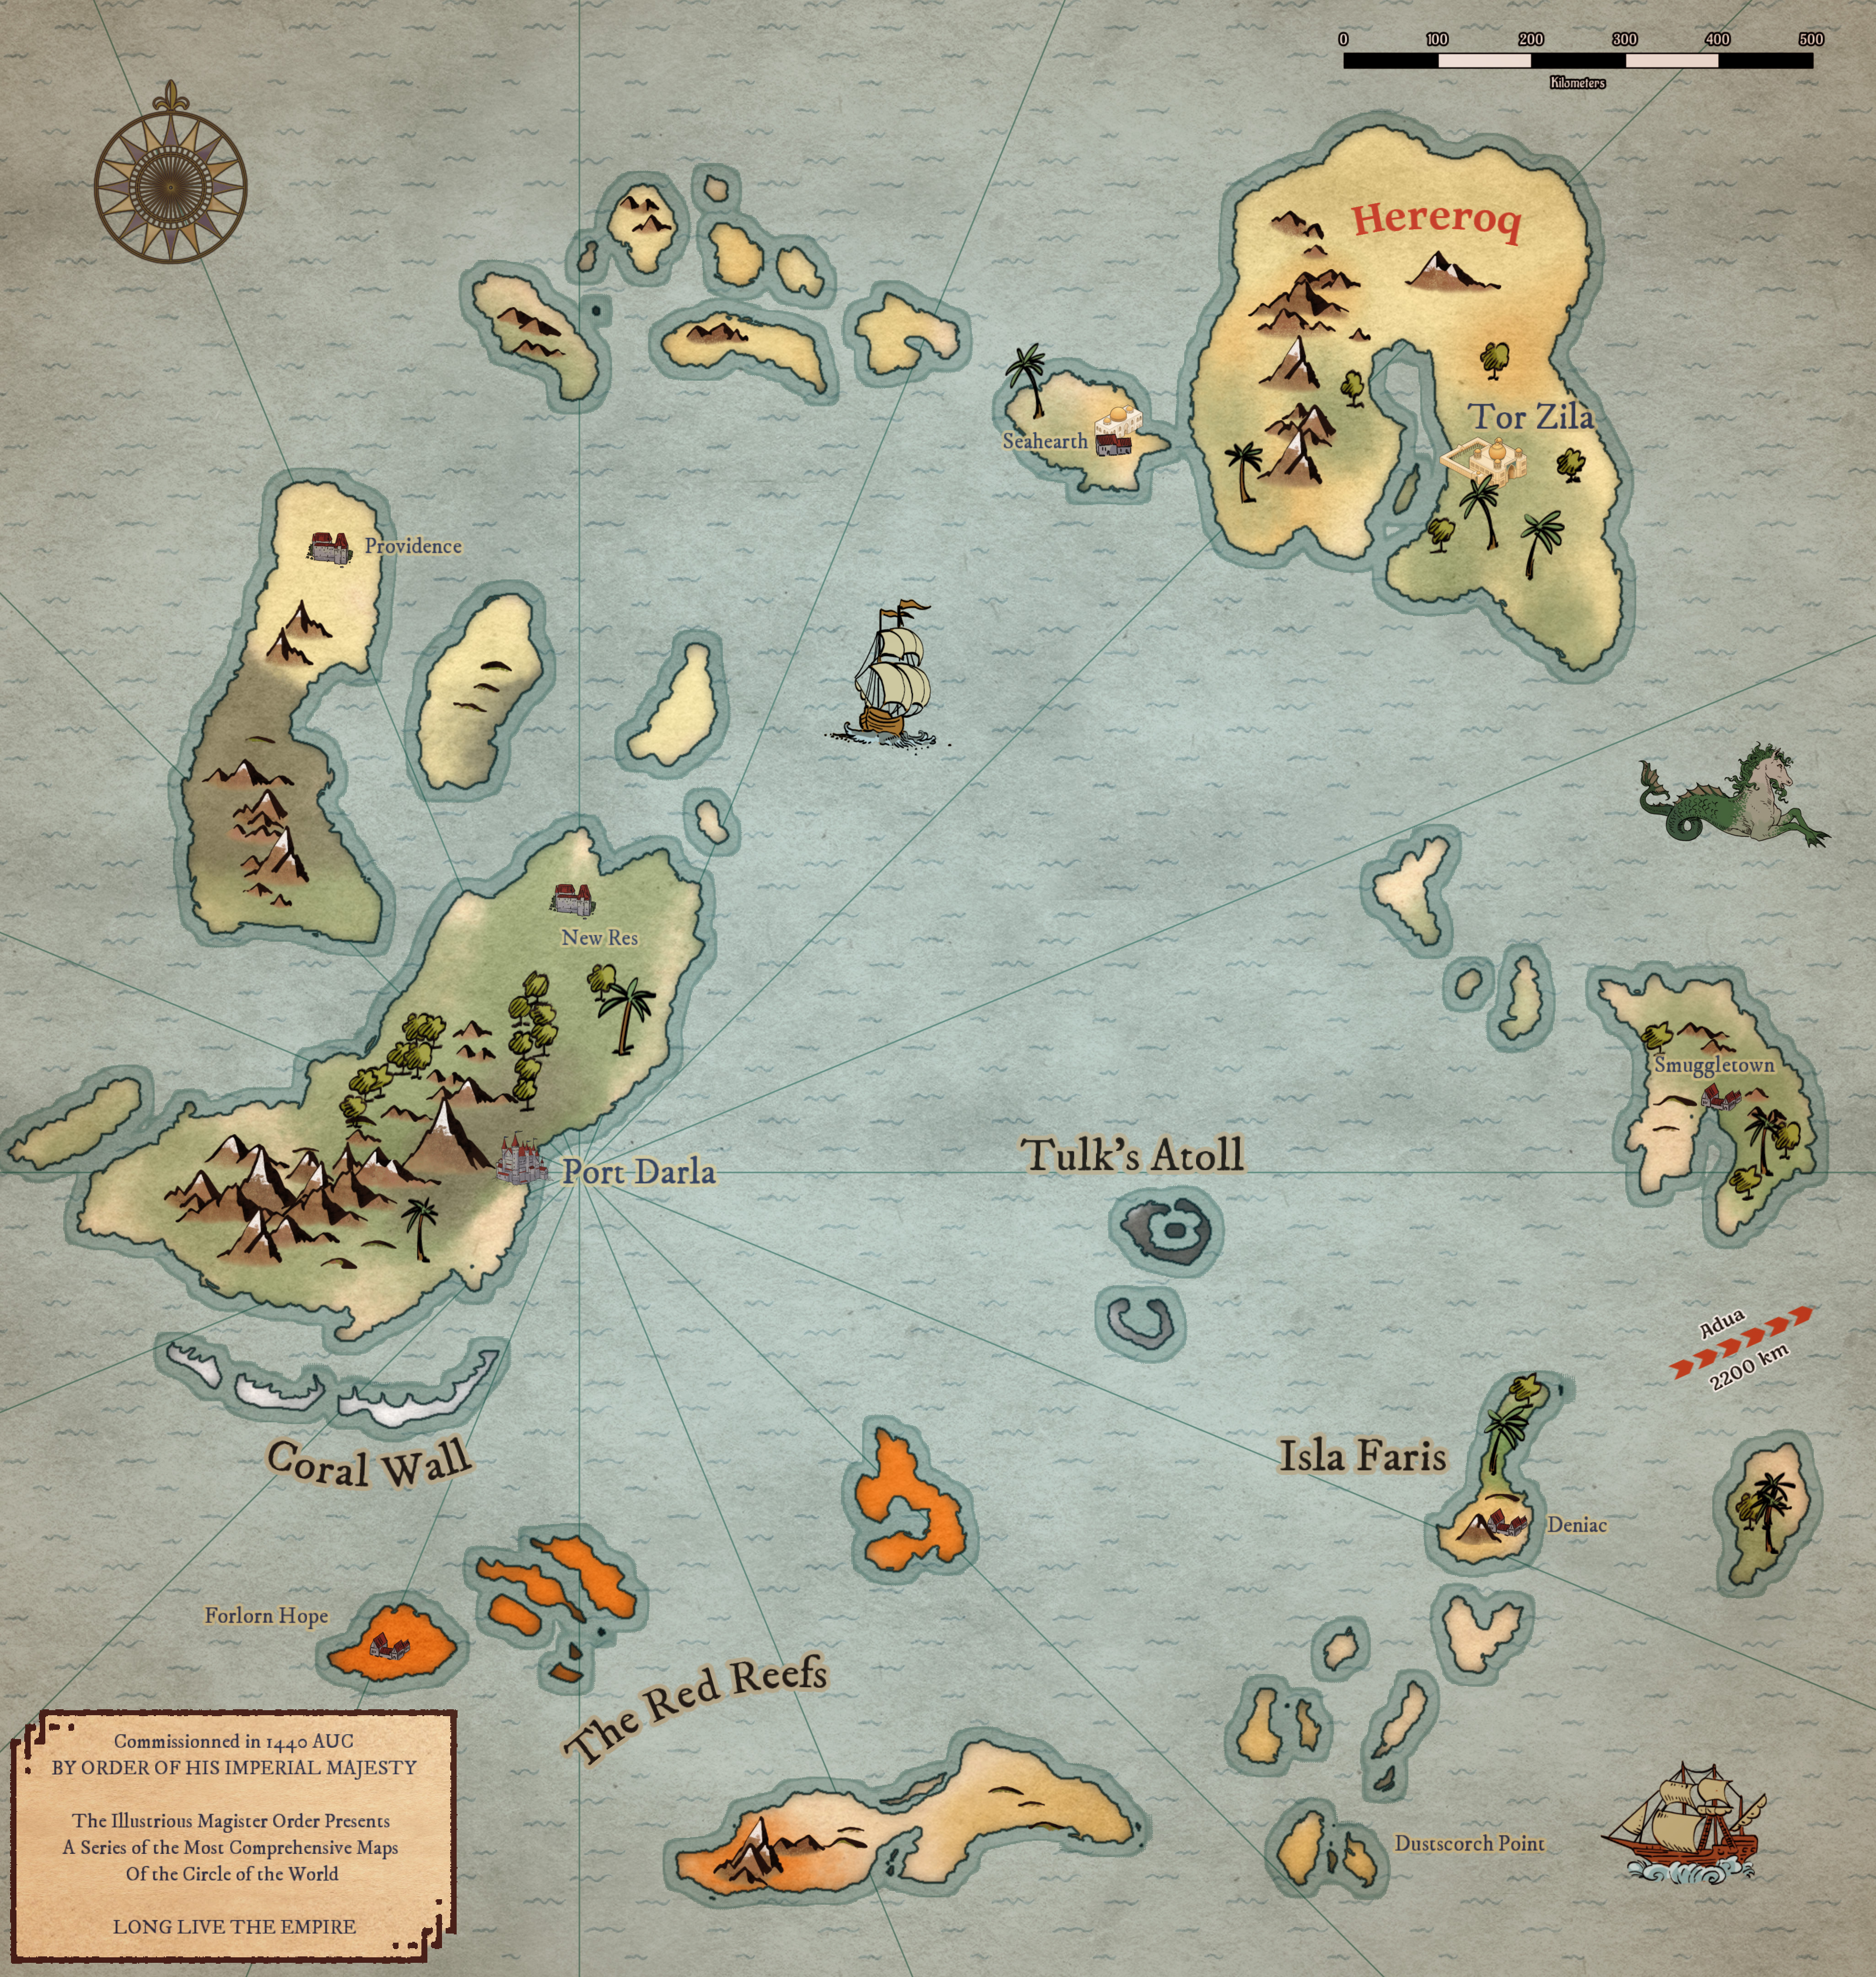
\includegraphics[angle=0,origin=c]{img/map_dreamshard.jpg}
    }
    \caption{Map of the Dreamshard Archipelago. Only major settlements are represented.}
    \label{map_1}
\end{figure*}


\begin{figure*}[ht!]
    \centering
    \resizebox{0.85\textwidth}{!}{
        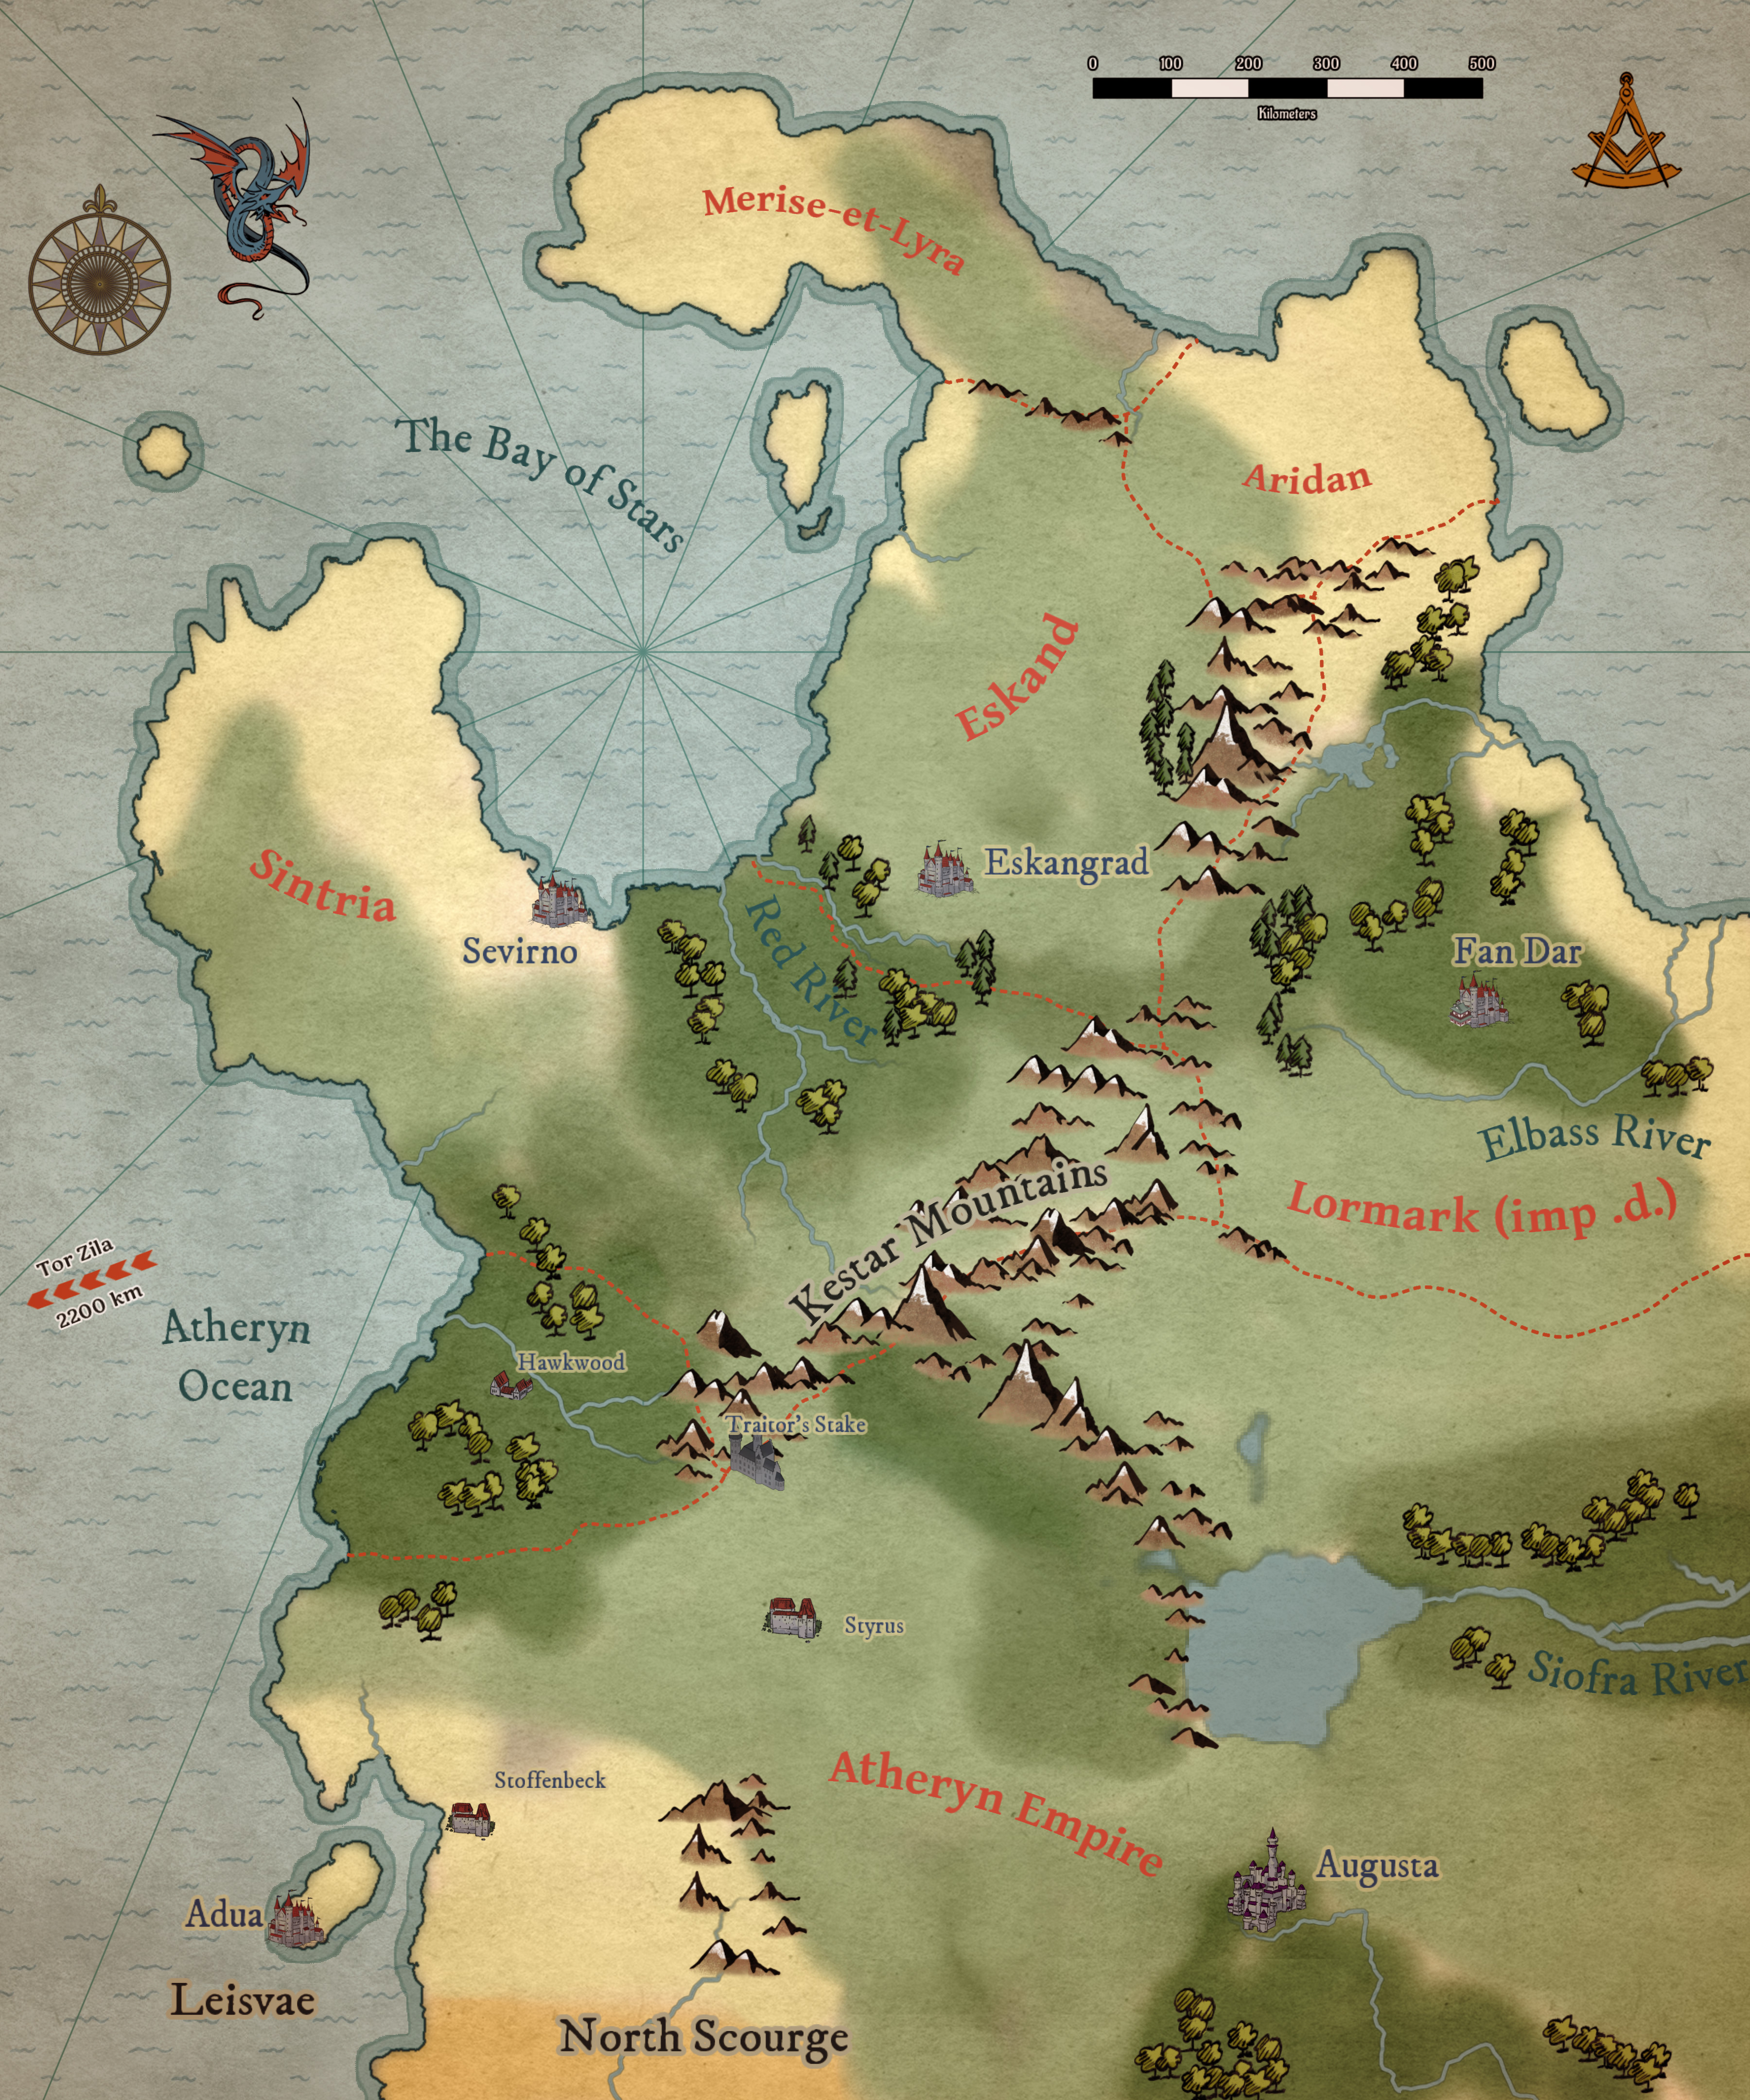
\includegraphics[angle=0,origin=c]{img/map_main_continent.jpg}
    }
    \caption{Map of the Eastern Realms, on the north of the Continent. Only major settlements and realms are represented. "Imp. d." stands for "Imperial dominion".}
    \label{map_2}
\end{figure*}



\subsection{Dreamshard Archipelago}

The Dreamshard Archipelago contains many large islands, some of which are contested by several parties. Its geography is presented on Map \ref{map_1}. It has a diameter of roughly 1800 kilometers, and its eastern edge is located about 2200 km from the western edge of the main Continent. As such, travel between the two takes about two weeks on average, depending on the weather.

The largest island of the archipelago is home to Port Darla, its greatest and msot important city. The secon largest island, to the northeast, constitutes the homelands of the realm of Hereroq. There are many smaller islands, including the warm and volcanic Isla Faris to the southeast, and the fertile island of Providence to the west.

Owing to its size, the Dreamshard covers a breadth of latitudes, and as such virtually every climate can be found within. That being said, the most widespread biome is similar to the Mediterranean climate in the real world: warm, with occasional dryness (especially in the southwest and northeast). However, the southern islands have a hot tropical climate, milder climates are found in the northwest, and many mountain ranges are high enough to have a cold climate.

The archipelago in rich in many important resources. Most are mainly of commercial interest, like spices and olives. But the Isles are also also particularly rich in tellurium, a metal critical to industrial applications of Magic.

Historically, the archipel has been settled for a long time. But it has seen renewed attention recently, with the latest wave of settlements (from the IDC, FSN, etc.) beginning only roughly a century and a half ago. It was justified, on paper at least, by the pursuit of old \textit{de jure} territorial claims. Even so, the polities of the archipelago remained a distant second fiddle in world affairs, until an uptick in the rate of discovery of Voskari artifacts resulted in a regain of interest and thus a settlement rush, 75 years ago.



\subsubsection{Port Darla}

Port Darla is a boom town, and contains headquarters of the Imperial Dreamshard Coumpany. It was founded by Francis Darla 62 years ago, with Lucius Clarence arriving as governor 4 years ago. 


\begin{rpg-quotebox}
    The advantage of having deep pockets? You can bury your opponents with their contents. \\ \textendash \textit{Lucius Clarence}
    \end{rpg-quotebox}
 
It has become an important city of thirty five thousand inhabitants, mostly funded by commerce incidental to the Dreamshard Rush. As a new city, it was built according to a geometric plan, with four main avenues corresponding to cardinal points.


\subsection{Eastern Realms}

The main continent, presented on Map \ref{map_2}, is home to several polities. It is often referred by its inhabitants simply as "the Continent", capitalized, in an amusing display of chauvinism. It is indeed large, even when only considering its northern part: the distance between Sevirno and Augusta is roughly 1600 km in a straight line.

The most notable polities of the Continent are: the powerful Atheryn Empire, the independant Northern Kingdoms, and the semi-independant Lormark valley. It has a temperate cold climate to the north of the Kestar mountains, while the south has a warmer climate.

The extreme south and east of this continent, which are not depicted on the map, remain only partially explored by the aformentioned polities. As such, they are improprely called the Uncharted Lands\footnote{In concept, this is a blank canvas for players to propose any origin concept they want, in accordance with the GM.}. They include (but are not limited to) the Scourge, a dry steppe full of aggressive cultures; This separates the so-called Eastern Realms from other advanced civilisations on the two other continents, because it lengthens the required sea travel as there are fewer safe harbors.

\section{Cosmogony}

The planet is a sphere, has one moon called Sela, and orbits a yellow sun simply called Sol. Known planets in the solar system include Lyria and Aulcus, and known constellations visible from the Dreamshard include the Chimera and the High Cross, which contains the Polar Star.

In the classical Atheryn Imperial calendar, used in the Northern Hemisphere, the year begins with spring and is divided in 12 months (Germinal, Bloomal, Landfall, Messydor, Sundary, Fructider, Vendemare, Brumare, Frosmare, Snowfall, Rainfall, Windfall) of 30 days each, plus an "out-of-calendar" week that celebrates the end of winter and the beginning of spring for this hemisphere. The first year of the calendar is the day of the founding of Augusta, the imperial capital. \textit{The current date is 18 Vendemare, 1440 A.U.C.}


\subsection{Magic}

\label{magic_lore}

Magic is a force that lets its practitioners achieve all sorts of effects, some of which bend the laws of physics as we know them in the real world. As best as anyone can tell, the existence of Magic seems to be a fundamental property of the universe. The currently prevailing theory is that sentience, in its broadest meaning, is what lets someone effect Magic.


\paragraph{Of Wizards and Magisters}

Magical potential is a combination of nature and nurture. This means that, technically, everyone can perform Magic. In practice, however, wizards are an extreme rarity\footnote{About as frequent as champion athletes, virtuoso artists, genius scientists, etc. are in the real world.}! This is because Magic is extremely difficult, and has a poor cost-to-benefit ratio for most people: it takes the average person years to learn how to conjure a small flame, while rubbing flints together is easy.  But for those with the natural capabilities (or money) to persevere, the rewards can be great. People who manage to push past the break-even point are called Wizards, with the very best being known as Magisters.


\begin{rpg-quotebox}
   The fewer people are capable of stopping you, the more powerful you are. \\ \textendash \textit{Arch Lector Merivahn}
\end{rpg-quotebox}

There exists a Magister Order which is meant, on paper, to be an association of those mighty few. But in practice, Magisters are almost completely autonomous. While collegial Institutes of Magic exist, in practice there are so few skilled Magic users that most Wizards learned through a more personal master-disciple relationship, or simply by trial and error. 

However, there are puzzling exceptions to these rules. Some people can have instinctive capabilities for Magic. Those are usually people with considerable Resolve, and in general what we would call Great People, Leaders and Heroes. For instance, consider Saint Lucien, a prominent figure in the Dawning War, which is the founding event of the Atheryn Empire. He became a powerful, if specialized, Magister with only minimal training. But he was a charismatic leader, and it was observed that his followers would often survive wounds that should have killed them. It goes without saying that this fueled intense jealousy from the Magisters.

Relatedly, the beliefs of many people, even without magical talent themselves, can still coalesce and produce magical effects or strengthen a Wizard. But in these cases, the effects are usually much more subtle. While gods do not exist in this setting, this effect led some people to see Magic as a divine gift (some believe it is from the Voskari...) or an answer to prayer, or something akin to unleashing one's "inner potential".

Parenthetically, while people with temporal power (kings, etc.) are expected to have a basic understanding of Magic, few use it themselves\footnote{Much like advanced technologies in the real world.}. Magister Kings are a terrifying sight, but since ruling can be a dangerous profession, most Magisters are content with acting as grey eminences instead of making plays for the throne.



\paragraph{On Source}

Magic is studied scientifically by some, but remains poorly understood. Tangentially, this explain the screwed-up formulation of prophecies and certain Spells: they are written by trial and error, modifying them a word at a time to see what best matches the currents of Magic. 

All the realizations discussed above led to the Source Theory of Magic: that Magic is created by \textit{sentience}, as Humans are by far the best generators of magical energy. This is done consciously by Wizards, who use their Intelligence to channel Magic; not only the magic generated by their own sentience, but also to a lesser degree channel the general "magical field" comin from the mere existence of sentient beings. The rest of mankind can do this unconsciously, but much less efficiently. There is only one flaw in this theory, but it is a major one: it appears non-sentient animals, golems, and even a barren desert will have a small but nonzero level of Source present. In fact, the cosmos itself contains endless Magic, but with minute density. No satisfactory theory currently explains why.

Raw Magic can be stored in physical form. It's usually in this form that is it called "Source", unsurprisingly. Source behaves something like a gel, but its behavior consistently defies the laws of physics. However, it is not usable as-is, and must be refined again through a Sigil to be effective.


\paragraph{The Nature of Magic}

Magic is performed through the proper Sigils, augmenting them with Accents. Each Sigil covers a certain type of effect, such as fire, healing, divination, to name a few.

The most common way to do so is by engraving or painting a Sigil on a support, with advanced inscribing requiring specialized materials and tools. Sigils can also be encoded in a vibration, such as a song, but the usual way to cast a Spell directly is by forming a Sigil through hand gestures. Experienced Wizards can be discrete and cast directly from their willpower without gestures or materials, but This is considerably more difficult. 

The main factors limiting the potential of Magic are intrinsic: Sigils and Accents must be made with daunting precision to work, and they are extremely difficult to standardize since the flow of Source is never exactly equal between two castings, even at the same position or the same time. This means that the most common way to use Magic is to use Magical Implements of pre-prepared Spells.

Indeed, some forms of technology rely on Enchanted Objects. While still rare, this is gaining popularity, but only up to an extent since this is very costly. As such, the practice has only noticeably impacted some specialized high-value industries.


Tangentially, even more potent Magic can be created by working at a more fundamental level through the Source Sigil. This is however enormously difficult and very finicky, and as such is not available to the players. It should be a "plot device" only if needed.

Based on Source Theory, it is also possible to Purge someone or something to extract their Source and strengthen Magic, but this is obviously frowned upon by most.


\paragraph{Effects and limitations}

\label{magic_effects}

While Magic can have many wondrous effects, it will remain fairly limited in scale. In particular, I would refer you to the description of the different Sigils, which is given in section \ref{abilities_list}, to get a general idea of what is possible. In this section, I will give additional clarifications.

In terms of scale, for instance, conjuring fireballs is extremely rare, and magical healing will usually be restricted to immediate knitting of the flesh and accelerating natural recovery. Magisters can be powerful, but nobody is strong enough to call down meteors or similar cataclysms. At least, that we know of... On that note, only Magisters can acheive anything really spectacular: for example, then tend to live longer, but mostly decades and not centuries\footnote{An apocryphal writing by Saint Lucien states that he ended up befriending families instead of individuals, justifying it by saying that "I befriend people I like, but sometime people change. Similarly, descendants are close but not quite their forebearers. I see no meaningful difference in either evolution."}.

Prescience through Divination is possible, but the usual form is simply a predictive algorithm that taps into the subconscious computing power of the caster's mind. Extralucid perception is however possible, by using this Sigil to talk to animals, in other languages, and for remote communications (although such long distance communications are difficulty and reserved for essential messages).

Sigils such as Nature or Summoning may be used for limited metamorphosis and mutagenic purposes, but any use of Summoning will have very impermanent results, as conjuration of physical matter out of nothing is extremely limited. It is also possible to be creative: for example, Telluric and Force have many engineering applications.

On the end of the spectrum, it should be noted that manipulating fundamental properties of space-time, the cosmos, and creating new planes of existence are all theoreticaly possible with the Source Sigil, the immense amounts of power required are well out of reach. For the moment, at least...

\paragraph{Echos}

Echos are remnants of sentient beings, a magical fac-simile created by the residual impact of their sentience. They manifest as disembodied ghosts. Echos can physically affect the real world in the world, but are usually very weak, unstable and nowhere near as smart as the alive person. When someone is still alive, their Echo does not manifest as it is (usually....) drowned out by the footprint of their current self\footnote{Incidentally, some random Echos found in the Aetheral suggest the existence of other sapient species far away, perhaps on another plane of existence. At least some of those Echos could be from our Earth, could they not?}.

There are three cumulative factors that strengthen an Echo: having a high Resole in life, being talented at Magic, or simply being manually "infused" magically in the proper way (although this is a risky and failure-prone procedure).

\begin{rpg-quotebox}
    From across time and space, they will answer the call. \\ \textendash \textit{Arch Lector Merivahn}
\end{rpg-quotebox}
        
Views on Echo manipulation views. Generally, people with a favorable view of Magic (mainly the Atheyn Empire and Lormark) will be open-minded. The others will be split between awe and wariness.




\subsection{Bestiary}

Most living species from the real world also exist here. There are, however, more than a few additions.

\rpgart{t}{img/art/kelp}


\subsubsection{Synthetics}

Any creature brought into being through artificial means (read: Magic) is called a Synthetic, often shortened to "Synth".

Magic can be a powerful mutagen. This means someone talented and determined enough can create truly screwed-up monstrosities. But creating something stable, or that can somewhat find its place in an ecosystem, both requires great power and great knowledge. 

Another drive behid the creation of Synthetics is that they can act as mataphysical Source reserve vats. As such, it should be noted that all Synthetics, without exception, have an intense craving for Source and Magic in all its forms.

As the fallout from many Voskari findings can attest, an uncontrolled release of Magic can also have this kind of effect.

As the voskari fallout attests, ambient uncontrolled release of magic being released can have this effect, introducing controlled or uncontrolled mutations 







\footnote{Genes can be selected for, creating specific family lines, epigenomics nonwitstanding. Indeed, Magisters are particulary adept at eugenics.}. \footnote{While natural evolution takes millenia, although microevolution of small characteristics can be done over a few generations (depending on generational speed)}


\footnote{Quadrupeds will generally share a bone structure and muscle attachments, traces of which can be seen in fish even. Main Muscle attachments for the face are cheekbones and lower far mandible (although scapula have different angles and first joint is closer to body, also share muzzle extrusion but with differing shapes ofc), beyond that chordata. Magic can be used to SPEED ALL OF THIS UP CONSIDERABLY.}


\paragraph{Constructs}


An important other aspect is the existence of Constructs, aka. golem and robots animated by magic, which are also technically "Synths". They can be partially organic or sometimes even fully inorganic. While those remain difficult to manufacture and hence rarely used, they are efficient calculators and can sometimes have some modest level of sentience. As such, those constructs are used to analyse large amounts of data and to perform hard labor. 


A philosphical dilemma is currently brewing on what moral status they should have.
Two other dilemmas : they are improving quicky and could conceivabley become fully sentient. As such, could they become wizards ? It is argued that their brand of sentience is focused on different applications, more specialized but dumber, compared to humans' and they are not focused on imitating humans but on high level mathematics, so this is uncertain. This is mere speculation. For now, at least... besides, artificial biological sapients are at least possible in principle, if rare :








\paragraph{Synthetic sapients}

The only naturally sapient race are Humans. Other sentients beings are so rare as to be anecdotal, and all of them are either whole-cloth Magical creations or simply magically-altered humans. 


Constructs are not sapient as we mentioned before, but the future is unclear.


\footnote{Artificial sapients are limited by the same biological constraints (brain maturation, etc.). Also, owing to the nature of their creation, they often have very unstable genomes (in the sense of containing many deleterious mutations and sometimes uneven numbers of chromosomes) ; as such, they are usually sterile or at least infertile.}



\footnote{Some Magisters even manufactured anthropomorphic human-animal hybrids for... sordid purposes.}


















\subsubsection{Menagerie}


- Put in some dinosaurs in a lost island ! (conserved magically ?) they also conveniently explain some "monstrous" creatures, just like IRL !

Off handedly mention that many of them can map to existing Bestiary profiles with only minor adjustments


Among the menagerie: to be spread into the relevant sections above when discussing them


\paragraph{Horrors}

- Animated trees
- Bismuth/tellurium golem
- Enthralling fungus
- Drowned ones
- Kraken (created)
- Arachnoid experiment
- Animated armor/Golem
- Drillworm? very large worm-ish thing
- Bone Bishop
- Drake purger
- Ashmen
 - Ghosts/echos
- "Demons" which are the result of Voskari experiments:	MANY, MANY fucked up Giger-esque Voskari-created monstrosities (ashmen included, and giger-esque machine tyrants) –> mentioned as "rumors"
- Constructs : golems, replicas
- Avatars: lupine anger, or avatars of strong emotions, works a bit like chaos demons in Warhammer 40k, and are close to Echos in their principle.

\paragraph{Success stories}



- There are however examples of artificial species that found an ecological niche. THey remain rare due to their craving for Source, but they exist nonetheless. 
	Shuddaka : trees with blue leaves and silver trunk, caused by the presence of actual silver, with communicating roots
	giant pillars-like coral formations
	coastal algae srpouting into the air thanks to air balloons
	monkey with a collar of sort of tentalcles for better prehension
	horses with boney crest for muscle attachment for additional strength
	large (mammoth-sized) animals with a flock of supporting organisms, killfish style
	basaltic organs are a must have! Idea: have some gradually slit tout, like missiles launching, and then explode in the air
	catlike species with very elastic tendons, can bend its spine into nighmarish contortions
	bird with mirror-like scales (yeah... I know) it can rotate while flying to reflect light or distract predactors
... as for size show a little of everything. i don't think i will go all the way up to something like massive dinosaurs, maybe one or two representants of almost extinct species, or an Abomination.






































\section{People and Cultures}

The world contains a variety of peoples and cultures, organized in a breadth of nations and polities. We will present those relevant to our story in this section.


In brief: the Eastern Realms, which designates the nations of the central Continent including the Atheryn Empire, have... heavily invested, shall we say, in the Dreamshard Archipelago recently. This, understandably, made the local potentates wary and had led to a sequence of portentous events. We will detail those later in section \ref{recent_history}).






- Describe skin tone and physical appearance of the peoples in their respective sections. Hereroq should be brown, lormark a bit more east-asian-ish but with high diversity, empire is mediterranean, north is european, find a bit more (notably there are blacks far to the south in a southern continent beyond the sand scourge, much like there is likely an eastern continent with asian-ish and brown-ish people







\subsection{Factions and History}

\begin{figure}[!ht]
    \centering      
        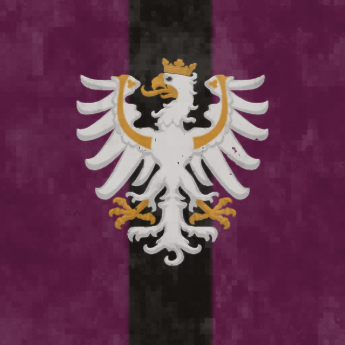
\includegraphics[scale=0.25]{img/flag/atheryn.png}
        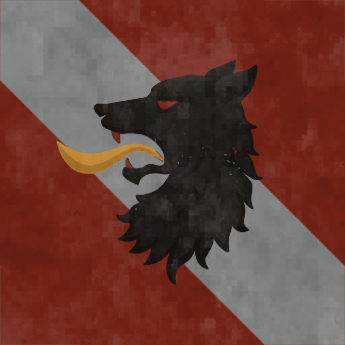
\includegraphics[scale=0.25]{img/flag/eskand.png}
        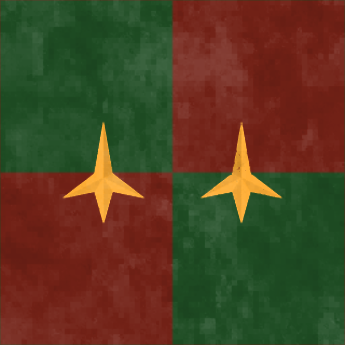
\includegraphics[scale=0.25]{img/flag/fnc.png}
        
\includegraphics[scale=0.25]{img/flag/fsn.png}
        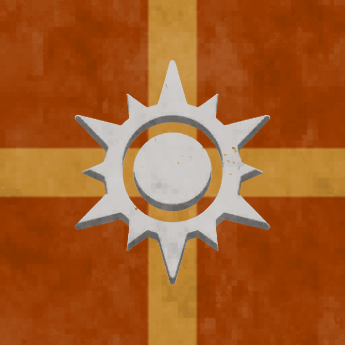
\includegraphics[scale=0.25]{img/flag/hereroq.png}
        
\includegraphics[scale=0.25]{img/flag/idc.png}
        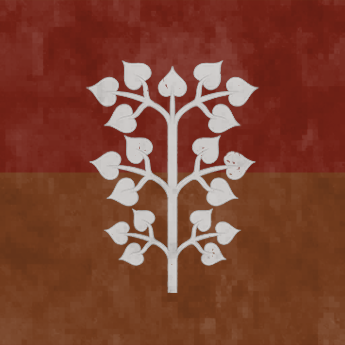
\includegraphics[scale=0.25]{img/flag/locals.png}
        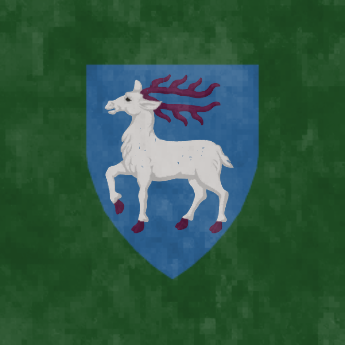
\includegraphics[scale=0.25]{img/flag/lormark.png}
        
\includegraphics[scale=0.25]{img/flag/sintria.png}
        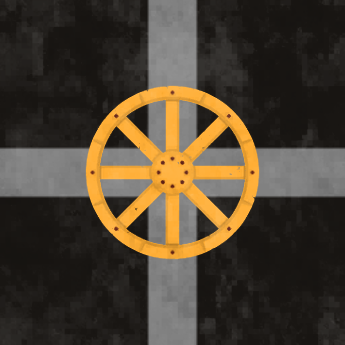
\includegraphics[scale=0.25]{img/flag/voskari.png}

    \caption{Flags of respectively, in classical reading order (left to right on each successive line, then moving in lines from top to bottom): the Atheryn Empire, Eskand, the First Northern Company, the Free Sailors Nation, Hereroq, the Imperial Dreamshard Company, the local Dreamshard dukedoms, Lormark, Sintria, the Voskari.}
    \label{flags}
\end{figure}








\subsubsection{Atheryn Empire}


A powerful empire ruling over the central part of the main Continent.


\textit{Leader}: Emperor Varen I Atheryn.

\textit{Population}: estimated 40 to 60 million inhabitants, 10 or more additional million with dependencies).

\textit{Wealth per capita}: Moderate on average, but with significant inequalities between the very rich elite class, and a considerable poor underclass. For dominions and dependencies, it is very variable.

\textit{Territory}: Most of the center of the Continent, with its capital at Augusta.
    
\textit{Colors}: Purple (major), white and black.


\begin{rpg-quotebox}
They say we make a desert and call it peace. I say we shatter so we can rebuild. \\ \textendash \textit{Gaël Valens-Détianne}
\end{rpg-quotebox}

The Atheryn Empire was founded by Saint Lucien in the Dawning War, which we mentioned previously. Their architecture style would best be described as neo-classical by the standards of the real world: they are very fond of columns and amphitheaters).

The Atheryn have grandiose ideas of what an Empire should be, straight out of the real-world Antiquity. The Atheryn believe they have been invested by the "Fates" of a grand civilizing mission, to bring the light of their culture, spread the "benefits" of their Empire to the entire world. As such, while they are somewhat racist, it is more of a cultural supremacism: they will embrace local converts and favor syncretism, as long as the resulting mix is more Atheryn than not, of course. On the flip side, defiance is met with brutal repression. 

Predictably, their political system is very backstabby. Although there is an Imperial Senate, senatorial mandates are very long, and suffrage is restricted to full Imperial citizens, making the system closer to an oligarchy than a democracy. That being said, as the Atheryn believe in their universalist principles, there are possible paths to citizenship.

As a result of this system, power tends to cluster in the hands of the Great Families of the Empire, including the <PUT NAMES HERE>. Unsurprisingly, they tend to be at loggerheads with each other. While open warfare is no longer the norm, they often employ covert operatives dubbed the Skiari. They are used against each other, and sometimes even against external threats, for a change.

It should be noted that despite the preponderence of Families, individuals can rise to power and found new Families themselves, inclusing by adoptiopn.
Despite Families individuals can rise, Caesar or Octavian style, and found families, inclusing by adoption
This makes it more meritocratic, as titles are not necessarily hereditary (in practice, heirs offten carry on, but despite all this oligarchy and heredity,  bureaucracy is powerful and often complicates the schemes of those above. It is not unheard of for bureaucrats to carve a sizable power base.

The Empire likes magic. Magisters are often cornerstones of the power structures and families. Indeed, the current Emperor, Varen Atheryn, is a skilled Magister, who poured funds into Apocrypha : university at Augusta, capital of the empire. While the Empire is very scientistic (not a misspelling, I mean they are attached to sciene) there is a not-insignificant part of the pop that sees the Voskari as demigods and worships them, causing some internal tensions. 


While the empire is the largest nation in the world, and regroups at present a good 25-30 percent of the planet's population, not all that population has the same culture. The Atheryn heatlands have exported the Atheryn language, administration, and a bit of their culture, but syncretism remains the order of the day in the empire, and ensures its relative stability. The Empire has vassal states and duchies with tenuous control, such as Lormark, or Leisvae island, a major commercial and tellurium mining centre, ruled by House Heim, recently suffering an attempted invasion by Eskand. (<-- this is mimbraine's imperial name, tell it to flo)


The Empire's fortunes have waxed and waned over the past millenia. The northern kingdoms of Sintria and Eskand broke off a good century or two ago. The Atheryn empire has recently suffered a rather large civil war, Vakir's rebellion (Vakir was Sintrian in origin) Now that Varen Atheryn has ramassé les dents of the Empire, it looks outwards again.  no internal wars in the empire now since it's done ramasser ses dents. See recent evets. Some famous regiments include 1st 'Black Cross', 7th 'Devil's Heart' and the 11th 'Chimera'

It should be noted that most of the Dreamshard is a \textit{de jure} part of the Empire, owing to early expeditions and treaties that are now centuries old and nobody cares about anymore except for paper-thin -- literally -- justifications, but it had attracted little interest and the locals were left to their own devices. Until now.



\paragraph{Imperial Dreamshard Company}

Short summary.

\textit{Leader}: Governor Lucius Clarence (it's complicated...)

\textit{Population}: 20K employees + 1.2 million Eastern colonists growing fast, plus a few million locals in the administered territories

\textit{Wealth per capita}: Moderate, but quickly improving.

\textit{Territory}: Port Darla and many isles

\textit{Colors}: Blue (major) and white (minor)


\begin{rpg-quotebox}
    "We shall bring civilization. Through the end of a musket, if need be."
    \end{rpg-quotebox}
    



The Imperial Dreamshard company, or IDC for short, is an ostensibly mercantile company founded under the authority of the the Atheryn Empire, of which most of the Dremshard Isles are a *de jure* part.

In practice, however, they behave more like conquerors. They are resolutely expansionist, and use their large fleet to assert their influence in the archipelago. They also take an active interest in the magical phenomena affecting the archipelago.

As an extensino of the Atheyn philosophy, many colonists have come settle the Dreamshard.


Note that The Imperial Dreamshard Company and FNC below are not simply extensions of their parent countries, they have some autonomy and disagreements with the mainland. Indeed, there is some politicking between Clarence the appointed governor who is a career bureaucrat, and Savian Détianne the Adjunct Minister in charge who got the job through connections



\subsubsection{Northern Kingdoms}

The two most noteworthy Northern Kingdoms are Eskand and Sintria. There are a handful of other smaller ones (see the map), but they are almost all in the sphere of influence of the big two. Usually Feudal, with heredity of titles, and a pyramid of nobles and no suffrage.




\paragraph{Sintria}

Short summary.

\textit{Leader}: Leto III Seinfeld

\textit{Population}: 11 million

\textit{Wealth per capita}: Moderate.

\textit{Territory}: a
    
\textit{Colors}: Yellow and white


\begin{rpg-quotebox}
    Quote \\ \textendash \textit{Source}
    \end{rpg-quotebox}


A cultural offshoot of the Atheryn, was a province three centuries ago but now independant. Some, but not much, hard feelings as a result. What really kicked tensions however is tha fact that Vakir (from the last imperial civil war) was Sintrian, hence tensions.

Architecture would be best described as modernized romanesque (renaissance)

They have been expansionnist, lately, both diplomatically and forcefully. The Empire worries they are trying to create a local sphere of influence that encompasses all the Northern Kingdoms.

As w would-be hegemon, Leto is weary of the developments in Eskand and is contemplating an expedition.
Sofia valskaya is secretly his illegiimate daughter, which complicates matters... see more in recent events in the red dawn


\paragraph{Eskand}


Short summary.


\textit{Leader}: King Harmach I (de jure, in exile), Lady Sofia Valskaya (de facto)

\textit{Population}: 6 million (uncertain due to recent troubles)

\textit{Wealth per capita}: Low, partly due to recent troubles.

\textit{Territory}: a
    
\textit{Colors}: Red (major), white and black


\begin{rpg-quotebox}
Quote \\ \textendash \textit{Source}
\end{rpg-quotebox}


Somewhat more rustic than its southern neighbors, Eskand used to be a junior partner in a personal union with Sintria under King Casamir III. Broke free 80 years ago, and has been in an uneasy peace with them, dotted with low-intensity wars under a variety of pretexts.
    

Architecture would be best described as brick gothic (use those exact terms)



Sofia Valskaya recently led a peasant rebellion that forced the king to abdicate in favor of noble who is a puppet of sofia. See recent events in the red dawn

\paragraph{First Northern Company}


Short summary.

\textit{Leader}: Director Alaria

\textit{Population}: approx. 15K employees + 750K colonists, growing, plus the locals in the administered territories

\textit{Wealth per capita}: High.

\textit{Territory}: Providence
    
\textit{Colors}: Red and green


\begin{rpg-quotebox}
"Enriching mankind and enriching oneself are not mutually exclusive goals."
\end{rpg-quotebox}


Counterpart of the IDC, Active In the Dreamshard. Sponsored by Sintria and Eskand mainly, but also significant participation from merchants from Lormark (see below).  
The FRC is not simply extensions of their parent countries, they have some autonomy and disagreements with the mainland, much like the IDC.

They seek Profit, profit, and perhaps even more profit. Relatedly, there are averse to interventionism and military adventurism ; their philosophy instead centers around establihsing trading posts as opposed to very large scale settlements.

Several Houses (close but not equivalent to families, in that it's not necessarily united by shared ancestry) vie for control of company interests.



\subsubsection{Lormark}

Short summary.

\textit{Leader}: Confederacy of city-states

\textit{Population}: 9 million, wealthier than average

\textit{Wealth per capita}: High, significant bourgeoisie.

\textit{Territory}: a
    
\textit{Colors}: Green and blue


\begin{rpg-quotebox}
Quote \\ \textendash \textit{Source}
\end{rpg-quotebox}

On paper, the Lormarkian principalties are grouped together as the Dominion of Lormark, which is a vassal of the Atheryn empire. However, the Empire takes a pretty lax approach and leaves them much autonomy, as long as they pay their taxes. Sometimes, they even remain in practice neutral in some imperial wars (although they join on paper). 

They are commerce focused, and are also an important cetner for the study of magic.

They have been known to (rarely ever since the empire control) wage the occasional low-intensity war between each other, though Imperial authority and the necessities of business usually demands an end to those quickly.

culture is  VERY cosmopolitan, and heavily influenced (founded ?) by foreigners. Architecture contains pagodas and stupas (use those terms I think) Due to being founded by settlers and merchant foreigners from the most eastern continent (and a few from the southern) and hybridizig with local cultures


The current emperor (Varen) is seeking to turn them into a unified puppet state with tighter control, which is not sitting well with them.

	

\subsubsection{Voskari}

Short summary.


\textit{Leader}: Arch Lector Merivahn, supposedly

\textit{Population}: Unknown. Likely select.

\textit{Wealth per capita}: Unknown. Likely spectacular.

\textit{Territory}: Unknown
    
\textit{Colors}: Black (major) and yellow


\begin{rpg-quotebox}
	"Is gratitude still germane when directed at the wrong person ?"
\end{rpg-quotebox}

A riddle wrapped in a mystery. Only few artifacts of them have been found, but findings are accelerating. The only tangible facts are the artifacts that share a common style and language. They share the Atheryn alphabet, but have their own language. Recognizable 19th-century stylistic elements mark them.

Artifacts belong to them about 10-20 years ahead of the current magical-technological level (not fantastically ahead, but quite advanced). The odd part is that this 10-20 years tech gap has remained constant ever since findings have begun, leading to speculation that they are still active and not an extinct civilization or an extinct Magister branch, and that they continue improving. One recurrent name : Merivahn.


If you buy into the most common theories, and according to some anecdotal evidence, here is the best state of knowledge: 
    - They are a world-domination Illuminati-ish secret society first and foremost. Speculated to be an ancestor or a splinter branch of the Magister Order (since magic is effective). Speculated also to be behind many weird magical phenomena recently observed.
    - external recruitment is possible from outside the organisation even though inside recruitment is preferred, and the total number of voskari Magisters is rather limited. Defections from the Voskari have happened, but the Voskari disinformation game is strong so people don't generally believe the defectors and stick to their own pet theory
    - There are two subfactions : the White and the Reds. They have competing visions for the future, and this War in Heaven is a heavy plot points. The exact nature of these competing visions is left for the reader-GM to decide.

Best we can tell, They are Humans, but that does not stop the fact that they are worshipped as mythical demi-gods in certain places. In fact The voskari religion (meaning cult that worships voskaris) is widespread and organized, which can generate religious tensions. They believe the leftover Voskari artifacts are "gifts" to mankind, to put us "on the right path". 


\subsubsection{Hereroq}


Short summary.


\textit{Leader}: Queen (closest corresponding title in Atheryn language) Hesria

\textit{Population}: estimated 14 million

\textit{Wealth per capita}: Low, but slowly improving.

\textit{Territory}: Tor Zila, Seahearth, all Isle of Hereroq and other dependencies.
    
\textit{Colors}: Beige and orange.


\begin{rpg-quotebox}
    "When the winds are changing, one must steer or die." \\ \textendash \textit{Hesria}
\end{rpg-quotebox}


The most noteworthy inhabitants of the Northern Dreamshard. A relatively large realm, controlling about half the total population and GDP of the Dreamshard Archipelago. While they shake hands with the Companies for now, the peace is tense and the Companies' outposts, including some of which are in Hereroq's dependencies, make the situation uneasy.

They are slightly backwards technologically compared to the Eastern Realms, but only slightly. Instead, their worst weakness is that they lack the wealth and especially the single-minded purpose of the Companies, which are attempting to extract concessions, buy shares in their economy, make "unequal treaties", ... and conquer what they cannot buy. They will need to play their cards rights in the coming storm. 

use some Moorish architecture too. mix of Turkic, Moorish and Mesoamerican features, with pyramids and large roof overhands (don't say ottoman and meso, say things like ("pointed arches for doors and columns, domes maybe (but many small domes instead of big ones, to be distinct), sandstone-ish, and meso-style pyramids with cyclopean blocks for religious purposes, maybe use the word "real-world moorish"))"

Notables are named the Sifs, which are member of un upper social class that is starting to diverge from the rest of the people. Politically, this is a federation: They are somewhat decentralized, with the Sifs ruling locally. Queen Hesria is looking to centralize more and reform to stand against the other Great Powers. Membership to the Sifs' social class is inherited, though, but it is reasonably frequent for rich or influential people to be named Sifs by the queen or by prominent Sifs. Also, culturally there is a 'right to rebellion', and for certain positions they have suffrage but it is censitaire. This means their values are somewhat meritocratic, but their social structure makes them quite traditionalistic and reactionary, and political corruption is a problem.

Religion is important (though the voskari cult is proportionally less important here than in the Eastern Realms, local traditions keep a better foothold), and self-sacrifice as well is a national virtue. Anecdote : they have a few temples with wings that are periodically rebuilt facing another direction, to symbolize the passing of time.

Strong tradition of naval exploration (they initiated contact with the main continent way back when, not the other way around) but don't really care for expansionnism, their last outposts have been taken over, first by the local dukedoms decades ago, and now by company encroachment (both by buying out, simply resettling them, and a few low-intensity wars). Trading posts of theirs, however, remain throughout the Dreamshard, and a handful on the Eastern continent. Importantly, they have a reputation for spycraft / being excellent spies.



Bayaz, a powerful magister, comes from here


\subsubsection{Free Sailors Nation}

Short summary.

\textit{Leader}: "Admiral" Veraume

\textit{Population}: approx. 10K sailors, + locals

\textit{Wealth per capita}: Moderate, but only in fungible and not productive assets.

\textit{Territory}: Smuggletown
    
\textit{Colors}: Green (major) and teal

\begin{rpg-quotebox}
    "Let the empires bicker. We'll be there, quietly waiting to bleed them dry." \\ \textendash \textit{Source}
\end{rpg-quotebox}


Pirates operating almost exclusively in the Dreamshard. Sometimes, some among their numbers sell their services as privateers. Some Asian-ish elements (junks, came as some early leaders were fleeing from the asian-ish lands and brought those ideas, and catamarans from ancient natives for scouting and messages) but very patchwork. 
	
Your garden-variety pirate nation, loyal to no one but themselves, seeking profit above all else. Open to taking privateer jobs. They are not, however, bloodthirsty thugs, but attempts to form an organized nation have been met with defiance from within.




\subsubsection{Local Dreamshard petty realms}


Short summary

\textit{Leader}: Various

\textit{Population}: Unknown, estimated at several million in total spread across the archipelago

\textit{Wealth per capita}: Low.

\textit{Territory}: Anywhere in the Dreamshard not (yet) claimed by any previously mentioned Great Power.
    
\textit{Colors}: a

\begin{rpg-quotebox}
    Sleepless nights are very good at reminding you about all you have to lose. \\ \textendash \textit{Who Said It}
\end{rpg-quotebox}

Besides the great powers, there are local dukedoms native to the isle, with wooden eastern european architecture. 
Many of them come from peaceful mixing between the "ancient natives" (see below) and very old progressive settlements from the Eastern Realms (who had some parts of dreamshard as de jure) ; however, their relative isolation led to cultural divergence, and today they are more like estranged cousins than brothers of the Easterners, especially with the mixing with the natives


Those dukedoms have intermediate level of tech, and relations with the Great Powers are tense because of encroachment. Alliances and low-level warfare between them sometimes, very shifting.
	Duchy names : Berus, Senria, add a third one

\subsubsection{Others}

There are scores of other people, big and small, that make up the Circle of the World.

Of note, we have:

- Ancient Natives of the dreamshard: pastoral, half-sedentary and half-nomadic (some tribes are only sedentary or nomadic while some alternatate ), with Chiefs that are a primus-inter-pares things and the influence of Druids/Shaman (dependin on translation), and the importance of Prestige. Skilled at raising camels and elephants for those living in the extreme south, while the northern ones are more often nomadic with horses or guerilla hiding in the forests, and the center ones have some wooden architecture. They are pretty much a spent force, have begun mixing in with the local dukedoms, particularly wiuth hereroq and now with the empire. Of no further consequence.

- Uncharted Lands are a border of the empire, like the limes in real life.
The Scourge is on the south of the main continents. Some parts are steppe, some parts are a dry dusty desert. Home to Steppe nomads.







\subsection{Local life}


\rpgart{t}{img/art/island}

The specificities of the culture of each faction have been mostly introduced in the previous section. Some additional considerations are presented here.

\paragraph{Languages}

The Atheryn language is a global \textit{lingua franca}, although it comes in a large variety of dialects, those are usually mutually intelligble. In particular, the languages spoken in the Northern Kingdoms are heavily influenced by it. Otherwise each culture has its own language.

\paragraph{Currency}

The money of the Atheryn Empire is the gold 'mark', subdivided in silver 'aces' and copper 'pennies', as stated in the rules. Ten pennies are worth an ace, and ten aces are worth a mark. Instead of marks, the North (and the FNC by extension) uses 'florens', and the Hereroqis uses 'denirs' which is often bastardized to 'deniers' by Easterners. All three have roughly equivalent value, and are generally seen as strong currency and accepted around the world.


\subsubsection{Technology}

The technological level is roughly equivalent to the Early Modern real world in Eurasia, outside of magic of course. with arquebus (in terms of philosophy, of course the presence of magic changes much) with forays into 18th century modern theories (or magical equivalents) but only rarely.


\begin{rpg-quotebox}
    Oh, we are way past 'unreasonable'. In fact, I'd say we crossed the line into 'insane' a while ago already. \\ \textendash \textit{Who Said It}
\end{rpg-quotebox}

proto-industrial revolution in the empire and the north with manufactures. As mentioned before, enchanted objects and magic have made in impact in some high-tech industries and there are applications, but it's very niche.

The best (often Voskari, but NOT EXCLUSIVELY! important to say Voskari do not have a monopoly on high-tech !!) can create some interesting stuff, which is partly technology and partly magical, but do recall that magic is studied by some people as a science so the frontier between the two can get blurry.



This includes, but is not limited to : primitive submarines, flying carpets, "omnicalculators" (often used to predict outcomes), magnetic rifles
Most of those, however, are limited series and prototypes. For now, at least...
- Needle gun (breechloader)
- Liquid breathing
- Enchanting, machine learning, 
- receptacle of energy upon a creature, to improve it ?
- Gateway/warp drive/wormhole ? Unsure





\subsubsection{Customs}

But also Tyranny antiquity-like "grandeur" and neoclassical thrown in for the Empire mostly

When it comes to what we would call today "progressiveness", meaning concepts such as female soldiers, homosexuality, and general acceptance, this world is arguably somewhere between the IRL Middle Ages in the Mediterranean, and today's Western societies. While opinions will of course vary by cultrure, in most of the world all of the above will be seen as "eccentricities", enough to stain a reputation but not sufficient to make someone a social pariah.

That being said, relations (romantic or otherwise) between social classes will be scrutinized in places where Great Families are important, and Magisters tend to be rather eugenist. Relatedly, I think a minor culture (not hereroq; likely one of the lormarkians) has castes (merchant, warrior, priest, peasant, etc.) somewhere

The Atheyrn Empire has indentured servitude, while the rest of the Eastern Realms instead use a lighter form of serfdom with potential for social mobility. Full-on chattel slavery is the exception, present only in a few polities in the world.

Furthermore the "do you not know that you are gods" religion is more popular in the north, while in the empire they have a deeper fascination with the voskari and the mystery-cults around them spring up there




Ship types:
	Like in PoE there should be Galleons and sloops, and dhows for hereroq.
	As for Junks, these are lormark based, but maybe the pirates adopted some. Same rasoning for the camataran-polynesian stuff like in pillars might be mentined in a Lormarkian background, but I am unsure it fits, perhaps pirates use them as messenger boats





\section{Recent history}

\label{recent_history}

In this section, I will present the most recent events and relevant \textit{dramatis personae}.

\subsection{Vakir's Rebellion}

The most important and portentous event in recent history is Vakir's Rebellion. Over the last century, the Atheryn Empire was experiencing a decline, which cultimated in the start of the Rebellion, 20 years ago. Vakir's Rebellion started with a dynastic pretext, and esclated when some families and even entire provinces that resented the Empire threw their lot with Karthus Vakir (who was originally Sintrian, but raised imperial, and had the backing of a portion of the army). Vakir's hold has been destroyed and is now Traitor's Stake.


\subsubsection{The Empire Strikes Back}

The Empire has now just recovered from Vakir's rebellion and is now looking outwards again. Emperor Varen Atheryn launched a reconquest of seceding territories 10 years ago that is nearing completion.

Emperor Varen Atheryn: knows magic. Held the empire together during the recent trouble, but his immediate family died in the war, so his nephew is now heir apparent. Due to this loss, Varen has grown jaded and disinterested.

One territory that escaped his notice is Leisvae. Invaded by Eskand during the rebellion, it was negelcted as the empire's resources were spent elsewhere and managed to liberate itself. Now jockeying between two factions led respectively by Caroline and Isgrin Heim, hesitating between rejoining the Empire and staying independant. Everybody awaits the empire's reaction

\subsection{The Red Dawn}

Meanwhile, in the North, a popular revolution called "Red Dawn" in Eskand led by Sofia recently deposed Eskand's king Harmach I and installed a puppet king. Leto III Seifeld of Sintria wishes to intervene. Sofia is secretly Leto's daughter and has been recorded saying that she "resents him for what he did" (unclear, assumed to have something to do with her mother). Leto is a benevolant despot, but a despot nonetheless. Tthinks he has a responsability to "make things right" for the North and build a sphere of influence for Sintira here. There is also the distinct fear that the Red Dawn could spread... which could explain Leto's motivatino to intervene.

\subsection{An Odyssey to the West}
 
Concurrently, there has been a quasi-colonization (use the word colonization !) boom in Dreamshard by all Eastern Realms over the last century, driven partly by escapism from the unstable situation in the East and by large increases in discovery of Voskari artifacts. This boom fed on itself, and now the archipelago became wealthy and valuable in and of itself, which increased its attrativeness even more.

Resulting in an uneasy political situation, as has been explained before when presenting the factions. It should be noted that many Dreamshard isles are historically fringe territories (explored and claimed on paper with sparse settlements) of many of the Eastern Realms, so they have a legitimate de jure claim, although they were negelcted backwaters until recently. This, however, has fooled precisely nobody. It is clear why exactly the settlers and the Companies are arriving (voskari artifacts, important resources, and well territory in general) and everybody knows the de jure claims are just a convenient excuse. After some diplomatic, economic, and even military skirmishing, there is now an uneasy peace between the Companies, Hereroq, and the other potentates.

\subsubsection{The City of the World's Desire}

In Port Darla : Lucius Clarence: 37yo, governor of the Imperial part of the Dreamshard Isles. Ambitious and sarcastic (rq : governor is an APPOINTEE position, he rose meritocratically here), nominated 4years ago. Lucius Clarence and the company's titular Minister (Savian Détianne) have a tense relationship as we mentioned, while Clarence is technically his supervisor, he has to negotiate sometimes to get full company backing. Mention Amelia Talborn as one of the Magisters who set up shop in Port Darla

Clarence and magister Bayaz are good friends


\subsection{A Farisian Question}

Which brings us to the most recent notable event, the eruption on Faris Island, in the Dreamshard Archipelago: pyroclastic clouds, weird sightings, suspected voskari involvement. Unexplained volcanic eruption as Isla Faris. Voskari artifacts found there. This has drawn the interest of everyone important.



---



\subsection{Some examples of names}

Don't make a list. Instead sprinkle them and mention them by name in the relevant sections about their origin cultures. say those are great families or persons of interest

A good way is to use them in the quotes

Empire > Some important people and families to name drop : Détianne, Savian, Arbuthnot, Lucius Clarence, Sabadi, Gael, Valens, Skiari ?, Berus, Zacharus, Du Bois, Talborn
HEREROQ > Some important people to name drop : Hesria, Lokdan, Nusal, Bayaz
North > Some important people and houses to name drop : Seinfeld, Val-Skaya, Anna, Mark, Talbot, Sevirno, Marda-Torai, Rieser
Lormark > Some important people and houses to name drop : Harmaak, Senria, Lu Dar, Radishaj
Voskari: Merivahn

